\documentclass[a4paper]{jsarticle}

%======================================================================
%		論文のタイトル,著者,日付
%======================================================================

\title{\Huge 光伝送工学\\\huge 第2回レポート\vspace{120mm}}
\author{\Large 濱崎 直紀\\\large (学籍番号:28G19096)\vspace{25mm}}
\date{令和元年11月27日}

%======================================================================
%		マクロの読み込みとコマンドの定義
%======================================================================

\usepackage{graphicx}       % eps fileを張り付けるのに必要
% \usepackage[dvipdfmx]{graphicx}     % png等の画像を貼りつけるのに必要
\usepackage{amssymb}
\usepackage{bm}     % 太字を書くのに必要
\usepackage{here}       % その場所に画像を入れるのに必要
\usepackage{comment}        % コメントを挟むのに必要
% \usepackage{listings}      % ソースコードを表示するのに必要
% \usepackage{jlisting}       % ソースコード内に日本語のコメントアウトがある場合必要(TEX Liveの場合,別途ダウンロードが必要)

%======================================================================
%		本文
%======================================================================

\begin{document}

\begin{titlepage}
\maketitle
\thispagestyle{empty}
\end{titlepage}

\begin{itemize}
    \setlength{\itemsep}{5mm}
    \item[1)] 
    \begin{eqnarray*}
        K=\frac{1-|S_{11}|^2-|S_{22}|^2+|\Delta|^2}{2|S_{12}S_{21}|}
    \end{eqnarray*}
    \begin{eqnarray*}
        |\Delta|=|S_{11}S_{22}-S_{12}S_{21}|
    \end{eqnarray*}
    よって,それぞれに値を代入して$K=0.878$, $|\Delta|=0.447$となる.\\
    \\
    \textcircled{\scriptsize1} $\frac{1-|S_{11}|^2-|S_{22}|^2+|\Delta|^2}{2|S_{12}S_{21}|}$\\
    \textcircled{\scriptsize2} $|S_{11}S_{22}-S_{12}S_{21}|$\\
    \textcircled{\scriptsize3} 0.878\\
    \textcircled{\scriptsize4} 0.447

    \item[2)]
    入力側において$\Gamma_s$の安定円の中心を$C_s$,半径を$r_s$とすると
    \begin{eqnarray*}
        C_s&=&\frac{(S_{11}-S^*_{22}\Delta)^*}{|S_{11}|^2-|\Delta|^2}\\
        &=&-9.12+j7.49\\
        &=&11.8\angle 140.6^\circ
    \end{eqnarray*}
    \begin{eqnarray*}
        r_s&=&\frac{|S_{12}S_{21}|}{||S_{11}|^2-|\Delta|^2|}\\
        &=&10.9
    \end{eqnarray*}
    となる.
    次に出力側において$\Gamma_L$の安定円の中心を$C_L$,半径を$r_L$とすると
    \begin{eqnarray*}
        C_s&=&\frac{(S_{22}-S^*_{11}\Delta)^*}{|S_{22}|^2-|\Delta|^2}\\
        &=&0.874-j2.80\\
        &=&2.93\angle -72.7^\circ
    \end{eqnarray*}
    \begin{eqnarray*}
        r_s&=&\frac{|S_{12}S_{21}|}{||S_{22}|^2-|\Delta|^2|}\\
        &=&3.77
    \end{eqnarray*}
    となる.\\
    また
    \begin{eqnarray*}
        |S_{11}|=0.496<1\\
        |S_{22}|=0.256<1
    \end{eqnarray*}
    より,$|S_{11}|$,$|S_{22}|$がともに1より小さいことから,原点を含む領域が安定となる.\\
    $\Gamma_S$, $\Gamma_L$の領域をそれぞれ図2,図3(レポート末尾に記載)に示す.\\
    \\
    \textcircled{\scriptsize5} 11.8\\
    \textcircled{\scriptsize6} 140.6\\
    \textcircled{\scriptsize7} 10.9\\
    \textcircled{\scriptsize8} 2.93\\
    \textcircled{\scriptsize9} -72.7\\
    \textcircled{\scriptsize10} 3.77\\
    \textcircled{\scriptsize11} 含む\\
    \textcircled{\scriptsize12} $|S_{11}|$\\
    \textcircled{\scriptsize13} $|S_{22}|$

    \item[3)]
    有能電力の定利得円について,安定円の中心を$C_a$,半径を$r_a$とする.\\
    $G_A=13{\rm db}=10^{\frac{13}{10}}$より
    \begin{eqnarray*}
        g_a&=&\frac{G_A}{|S_{21}|^2}\\
        &=&1.32
    \end{eqnarray*}
    \begin{eqnarray*}
        C_a&=&\frac{g_a(S_{11}-\Delta S^*_{22})^*}{1+g_a(|S_{11}|^2-|\Delta|^2)}\\
        &=&-0.525+j0.431\\
        &=&0.680\angle 140.6^\circ
    \end{eqnarray*}
    \begin{eqnarray*}
        r_a&=&\frac{\sqrt{1-2Kg_a|S_{12}S_{21}|+g_a^2|S_{12}S_{21}|^2}}{|1+g_a(|S_11|^2-|\Delta|^2)|}\\
        &=&0.493
    \end{eqnarray*}
    となる.\\
    また,この円は有能電力利得が$\Gamma_s$の関数であるため,図2に描ける.\\
    \\
    \textcircled{\scriptsize14} 0.680\\
    \textcircled{\scriptsize15} 140.6\\
    \textcircled{\scriptsize16} 0.493\\
    \textcircled{\scriptsize17} 2

    \item[4)]
    \begin{eqnarray*}
        N&=&\frac{F-F_{\rm min}}{4r_n}|1+\Gamma_{opt}|^2\\
        &=&0.153
    \end{eqnarray*}
    \begin{eqnarray*}
        C_F&=&\frac{\Gamma_{opt}}{N+1}\\
        &=&0.115+j0.382\\
        &=&0.399\angle 73.3^\circ
    \end{eqnarray*}
    \begin{eqnarray*}
        r_F&=&\frac{1}{N+1}\sqrt{N^2+N(1-|\Gamma_{opt}|^2)}\\
        &=&0.330
    \end{eqnarray*}
    この円は雑音指数が$\Gamma_s$の関数であるため,図2に描ける.\\
    \\
    \textcircled{\scriptsize18} 0.399\\
    \textcircled{\scriptsize19} 73.3\\
    \textcircled{\scriptsize20} 0.330\\
    \textcircled{\scriptsize21} 2

    \item[5)]
    入力規格化インピーダンスは
    \begin{eqnarray*}
        z&=&\frac{1+\Gamma_s}{1-\Gamma_s}\\
        &=&0.606+j0.584
    \end{eqnarray*} 
    となり,信号源インピーダンスは
    \begin{eqnarray*}
        Z_s&=&Z_0z\\
        &=&30.3+j29.2
    \end{eqnarray*}
    となる.\\
    \\
    \textcircled{\scriptsize22} 30.3\\
    \textcircled{\scriptsize23} 29.2

    \item[6)]
    図4に示す整合回路をSmith V4.0を用いて設計すると,$C_1=1.6{\rm pF}$, $L_1=1.4{\rm nH}$となる.\\
    \\
    \textcircled{\scriptsize24} 1.6\\
    \textcircled{\scriptsize25} 1.4

    \item[7)]
    \begin{eqnarray*}
        \Gamma_{out}&=&S_{22}+\frac{S_{12}S_{21}\Gamma_s}{1-S_{11}\Gamma_s}\\
        &=&-0.179-j0.324\\
        &=&0.370\angle -118.9^\circ
    \end{eqnarray*} 
    また,
    \begin{eqnarray*}
        VSWR_{out}=\frac{1+|\Gamma_{OMN}|}{1-|\Gamma_{OMN}|}=2
    \end{eqnarray*}
    よって
    \begin{eqnarray*}
        |\Gamma_{OMN}|=\frac{1}{3}
    \end{eqnarray*}
    ゆえに
    \begin{eqnarray*}
        C_{VO}&=&\frac{\Gamma^*_{out}(1-|\Gamma_{OMN}|^2)}{1-|\Gamma_{OMN}\Gamma_{out}|^2}\\
        &=&-0.161+j0.292\\
        &=&0.334\angle 118.9^\circ
    \end{eqnarray*}
    \begin{eqnarray*}
        R_{VO}&=&\frac{|\Gamma_{OMN}|(1-|\Gamma_{out}|^2)}{1-|\Gamma_{OMN}\Gamma_{out}|^2}\\
        &=&0.292
    \end{eqnarray*}
    また,出力・定$VSWR$円は$\Gamma_L$の関数より図3に描ける.\\
    \\
    \textcircled{\scriptsize26} 0.370\\
    \textcircled{\scriptsize27} -118.9\\
    \textcircled{\scriptsize28} 0.334\\
    \textcircled{\scriptsize29} 118.9\\
    \textcircled{\scriptsize30} 0.292\\
    \textcircled{\scriptsize31} 3

    \item[8)]
    \begin{eqnarray*}
        \Gamma_{in}=S_{11}+\frac{S_{12}S_{21}\Gamma_L}{1-S_{22}\Gamma_L}
    \end{eqnarray*}
    \begin{eqnarray*}
        |\Gamma_{IMN}|=|\frac{\Gamma_{in}-\Gamma^*_s}{1-\Gamma_s\Gamma_{in}}|
    \end{eqnarray*}
    \begin{eqnarray*}
        VSWR_{in}=\frac{1+|\Gamma_{IMN}|}{1-|\Gamma_{IMN}|}
    \end{eqnarray*}
    なので,各$\theta$に対するそれぞれの値は表\ref{tab:VSMR}のようになる.
    \begin{table}[H]
        \begin{center}
            \begin{tabular}{c|cccc}
                \hline
                $\theta$ & $0^\circ$ & $90^\circ$ & $180^\circ$ & $270^\circ$\\
                \hline \hline
                $\Gamma_L$ & $0.131+j0.292$ & $-0.161+j0.584$ & $-0.454+j0.292$ & $-0.161-j0.0001$\\
                $\Gamma_{in}$ & $-0.484-j0.336$ & $-0.620-j0.560$ & $-0.390-j0.656$ & $-0.298-j0.463$\\
                $|\Gamma_{IMN}|$ & $0.467$ & $0.736$ & $0.549$ & $0.263$\\
                $VSWR_{in}$ & $2.75$ & $6.56$ & $3.44$ & $1.71$\\
                \hline
            \end{tabular}
            \caption{各$\theta$における$VSWR$}
            \label{tab:VSMR}
        \end{center}
    \end{table}
    よって$VSWR_{in}$が最も小さくなるのは$\theta=270^\circ$のときである.\\
    \\
    \textcircled{\scriptsize32} 270

    \item[9)]
    規格化負荷インピーダンスは
    \begin{eqnarray*}
        z_L&=&\frac{1+\Gamma_L}{1-\Gamma_L}\\
        &=&0.722-j0.0002
    \end{eqnarray*}
    よって
    \begin{eqnarray*}
        Z_L=Z_0z_L=36.1-j0.011
    \end{eqnarray*}
    ゆえに,図5示す整合回路をSmith V4.0を用いて設計すると,$C_2=0.397{\rm pF}$, $L_2=0.713{\rm nH}$となる.\\
    \\
    \textcircled{\scriptsize33} 0.397\\
    \textcircled{\scriptsize34} 0.713

    \item[10)]
    回路構成は図6のようになった.
    \setcounter{figure}{5}
    \begin{figure}[H]
        \begin{center}
            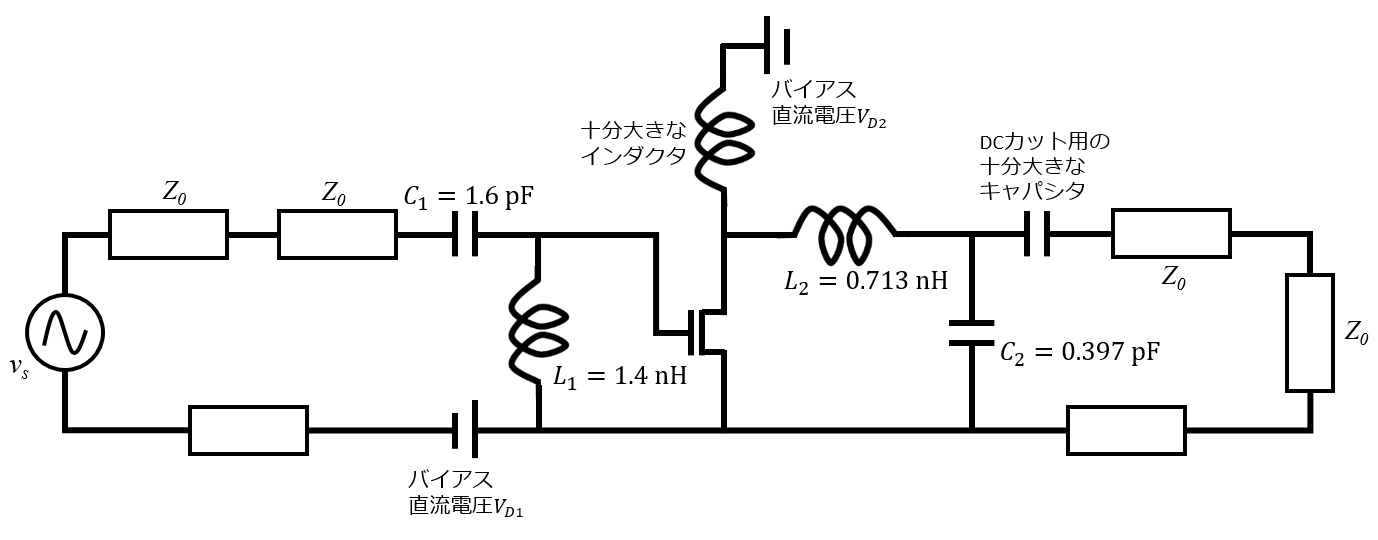
\includegraphics[width=150mm]{./figures/section/6.eps}
            \caption{}
        \end{center}
    \end{figure}
\end{itemize}

\end{document}